%%%%%%%%%%%%%%%%%%%%%%%%%%%%%%%%%%%%%
% Report template for COMP23111
% (2014-2015)
%
%	Alvaro A. A. Fernandes
%	Klitos Christodoulou
%
%%%%%%%%%%%%%%%%%%%%%%%%%%%%%%%%%%%%%

\documentclass[11pt,a4paper]{article}

% environment
\usepackage{fancyhdr} % this is needed to include headers
\usepackage{lastpage} % this is needed to include numbered pages
\pagestyle{fancy}
\usepackage{verbatim} % this is needed to include the SQL output
\usepackage{graphicx} % this is needed to include figures
\usepackage{listings} % this is needed to include the SQL output
\usepackage{epstopdf} % this is needed to include the EPS figure

% add a header consisting of your student ID and lab exercise number
\lhead{\textbf{ID:} 1234567}
\rhead{\textbf{COMP23111} - Lab Exercise N}
\cfoot{\thepage\ of \pageref{LastPage}}

% change the margins of the page
\usepackage[margin=0.6in]{geometry}

% set the parameters for the listings package
\lstset{
language=SQL,                           % Code langugage
basicstyle=\ttfamily,                   % Code font, Examples: \footnotesize, \ttfamily
}

% now set up a simpler command to wrap the inclusion of SQL scripts
\newcommand{\includesqloutput}[1]{\tiny \lstinputlisting{#1} \normalsize}

%%%% Start a new document
\begin{document}

% make sure that you change the next line to the correct exercise number
\title{\textbf{COMP23111} - Lab Exercise N}

% your full name goes here, and do not forget your student ID
\author{James, Peach \\ \textbf{ID:8974863} } 

% remember to copy this template and change the name of the file
% according to the rules in the Practical Sessions Manual

% now LaTeX prints the title, author name, etc. here
\maketitle
\thispagestyle{empty} % remove page numbering on first page
\newpage % start a new page

%%%
%  Create a new section and include the answer for each task as a subsection
%%%
\section{Part 1 - SQL Statements}

\subsection{A listing of the data \& structure of each table}
% include SQL output here, keep it in a separate file and include it here as the 
% example below.

\includesqloutput{sqlOutputs/LabEx1Out.lst}

%%%
%  Create a new section and include an ER diagram in .pdf format
%%%
\section{Part 2 - Example ER-diagram}

A Dia diagram is included below:

% Use the graphics environment to insert an EPS figure. Make sure that you scale it so that it fits.
% Also, consider using \newpage before and after in order to isolate it in a page.
\begin{figure}[!htbp]      
   	\centering
	\centerline{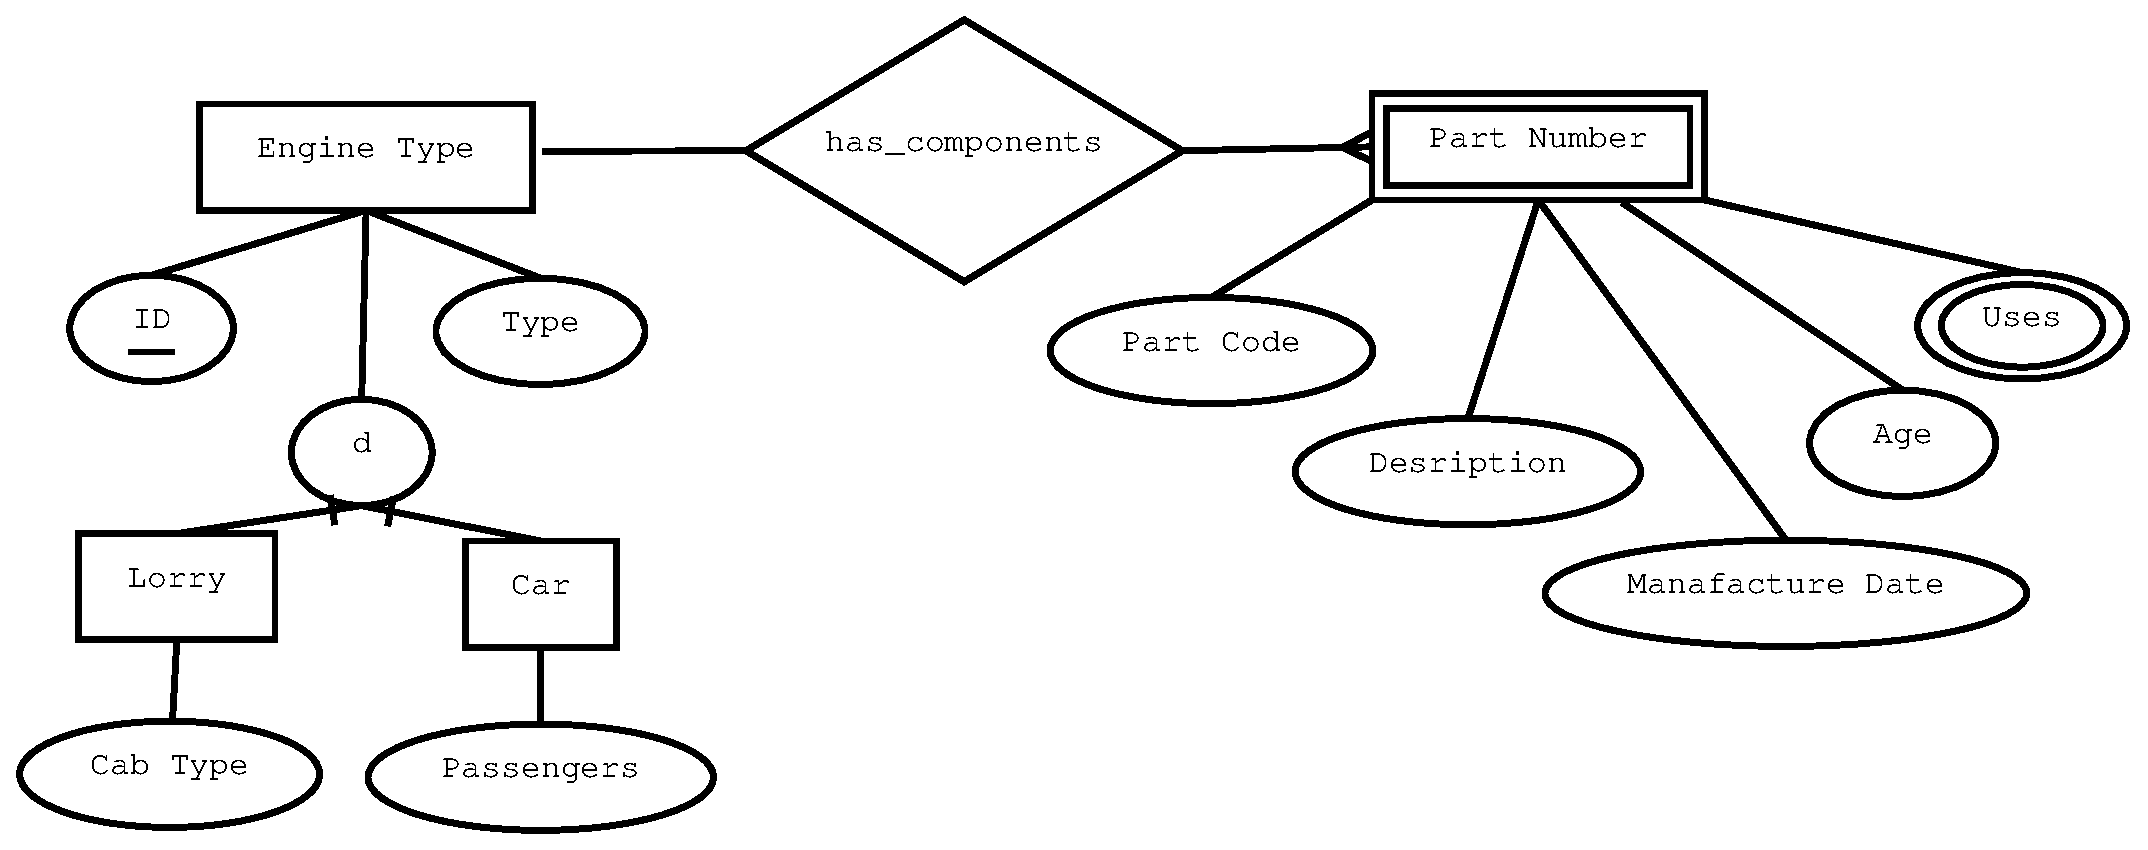
\includegraphics[width=0.75\textwidth]{./diagrams/AutoManafacture.eps}}
	\caption{Auto manafacture example ER diagram, created in DIA.}
	\label{fig:test-figure}
\end{figure}
\label{LastPage}
\end{document}
%%%% End document here
